\section{ICD in Clusters}

\subsection{NeAr Clusters}
\begin{figure}[h]
 \centering
 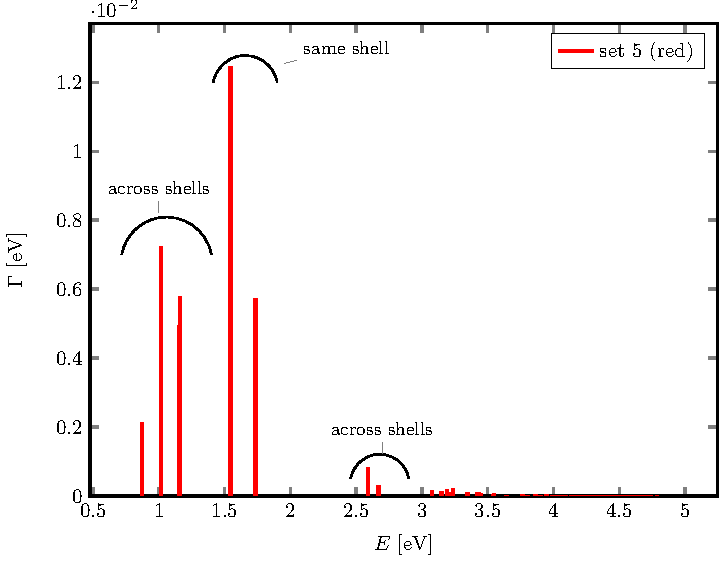
\includegraphics[width=\columnwidth]{pics/rot.pdf}\\
 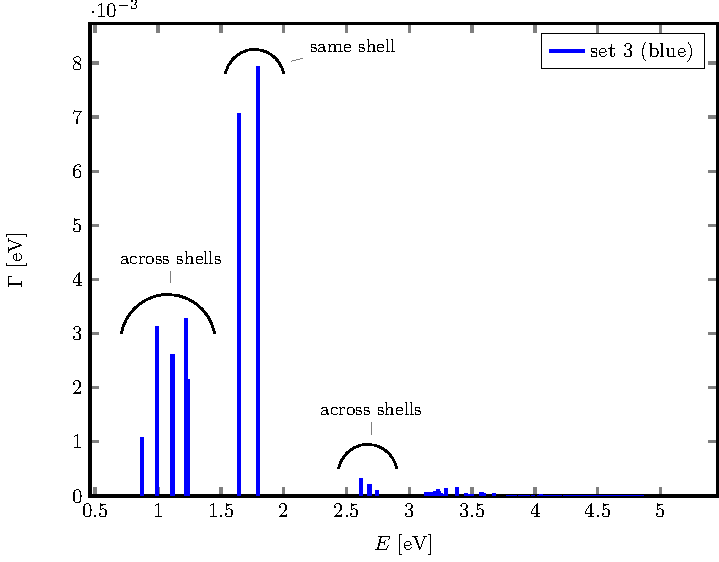
\includegraphics[width=\columnwidth]{pics/blue.pdf}
 \caption{ICD spectra for the NeNe-ICD part of the structures of set 3 and
          set 5 of the NeAr clusters in Ref. \cite{Fasshauer14_1}
          plotted as stick spectra.
          The different peak groups resemble different pair types
          within the NeAr clusters. The lowest energy peaks (\textbf{a})
          refer to nearest neighbours
          of different shells, the peak group \textbf{b} refers
          to nearest neighbours within one shell and the peak group \textbf{c}
          refers to next nearest neighbours between different shells.
          The peaks in group \textbf{d} contain both peaks stemming from
          pairs within the same shell as well as pairs consisting of atoms
          of different shells.}
 \label{figure:rot}
\end{figure}

%\begin{figure}
% \centering
% 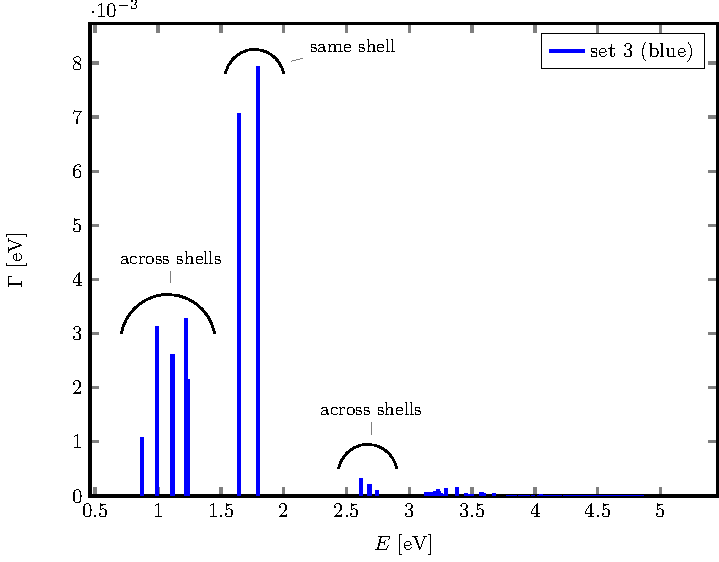
\includegraphics[width=\textwidth]{pics/blue.pdf}
% \caption{}
% \label{figure:blue}
%\end{figure}

\subsection{Icosahedral vs. fcc Structure of Clusters}
\begin{figure}[h]
 \centering
 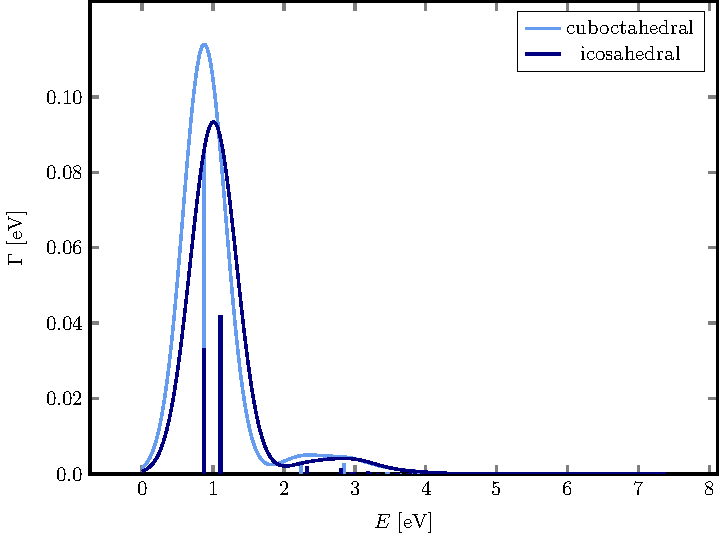
\includegraphics[width=\columnwidth]{pics/reinNe}
 \caption{ICD spectra of pure neon clusters consisting of 55 atoms in
          icosahedral and fcc structure. In clusters with an ideal fcc structure
          all interatomic distances are the same and hence only one peak
          for each shell around any atom in the cluster is to be expected.
          In ideal icosahedral clusters the interatomic distances between atoms
          within the same shell and between atoms in neighbouring atoms
          are different. Therefore two peaks for interactions partners
          at different distances can be expected. This feature might
          help to experimentally identify the underlying structure of clusters.}
 \label{figure:reinNe}
\end{figure}
